\customchapter{INTRODUCCIÓN} 

\introsection{Presentación del tema de investigación}
%%Preguntar si debería mencionar en el primer párrafo si hablar de por qué espacios cerrados y no espacios abiertos (mayor acumulación).
En los últimos años, la calidad del aire interior se ha convertido en un tema de creciente preocupación, especialmente en espacios cerrados como salones de clase. La relevancia de mantener los niveles de calidad de aire adecuados de interiores se justifica dado que la mayoría de personas pasan alrededor del 90\% de su  tiempo en estos ambientes \cite{its_about_time_a_comparison_of_canadian_and_american_time_activity_patterns}. Bajo este contexto, entre los principales enfoques de los sistemas de monitoreo de la calidad de aire en espacios cerrados desde el año 2015 están la medición y seguimiento de los niveles de CO\textsubscript{2}, los cuales se realizan en un 65\% de ellos \cite{IAQ_monitoring_systems_based_on_internet_of_things_a_systematic_review}. El interés por este parámetro de medición de la calidad de aire en espacios cerrados (IAQ: indoor air quality) se debe a la relación que hay entre los altos niveles de CO\textsubscript{2} y distintos efectos perjudiciales a nivel fisiológico y psicomotor \cite{effects_of_low_level_inhalation_exposure_to_carbon_dioxide_in_indoor_environments_a_short_review_on_human_health_and_psychomotor_performance}. Por este motivo, tanto organizaciones internacionales como nacionales han emitido regulaciones sobre los niveles de CO\textsubscript{2} en espacios cerrados. Por un lado, de acuerdo con la base de datos de la Sociedad Internacional de la Calidad del Aire Interior y Clima (ISIAQ: International Society of Indoor Air Quality and Climate), la cual registra las regulaciones impuestas por los gobiernos de los países del mundo afiliados, se registró que la moda del valor máximo permitido de CO\textsubscript{2} en interiores es de 1000 ppm; mientras que los valores más altos y bajos son 1500 ppm y 700 ppm, respectivamente \cite{indoor_air_quality_guidelines_from_across_the_world_an_appraisal_considering_energy_saving_health_productivity_and_comfort} \cite{ISIAQ_database}. Por otro lado, en el ámbito nacional peruano, la directiva administrativa n°349-MINSA/DGIESP-2024 señala que el umbral de concentración de CO\textsubscript{2} adecuado es 400 ppm sobre el nivel de base, es decir, la medición registrada en el ambiente sin personas; mientras que se señala que es deseable que no se sobrepasen las 1000 ppm \cite{directiva_minsa}. 

Este tema es de particular relevancia en ingeniería debido a la creciente adopción de tecnologías de Internet de las Cosas (IoT: Internet of Things) en diversos sectores, incluyendo el cuidado de la salud y la educación. El IoT constituye soluciones tecnológicas mediante la integración de sensores, actuadores y otros componentes de hardware en un mismo ecosistema que les permita interactuar entre sí o con una central para gestionar los datos adquiridos y ordenar las acciones requeridas \cite{the_application_of_internet_of_things_in_healthcare_a_systematic_literature_review_and_classification}. Este importante crecimiento en este tipo de soluciones está fuertemente ligado con otro concepto, las ciudades inteligentes. Este concepto surge como una propuesta para mitigar problemas generados por el rápido crecimiento de la población, la consecuente urbanización y el crecimiento de las sociedades; cuyo principal desafío es asegurar la interoperabilidad de tecnologías heterogéneas \cite{indoor_air_quality_assessment_using_a_co2_monitoring_system_based_on_internet_of_things}. En este sentido, las tecnologías IoT están directamente asociadas a ofrecer soluciones frente a al desafío de la interoperabilidad presente en las ciudades inteligentes.

Hasta la fecha se han realizado diversos estudios sobre el monitoreo de CO2 utilizando soluciones tecnológicas, ya sea mediante IoT o medidores de mano. En el caso de las soluciones que emplean IoT, presentan una estructura similar a la mostrada en la figura \ref{fig: estructura_general_IoT}, la cual se constituye de nodos sensores que se comunican con un servidor que almacena, analiza y muestra la información procesada. Este tipo de soluciones son principalmente utilizadas para un ambiente específico sobre el cual está desplegada la infraestructura de red, aunque bien podría ser escalable, no están pensadas para movilizarse constantemente a una variedad de ambientes. En contrapartida, existen soluciones como los medidores de mano de IAQ, cuyas principales fortalezas son la facilidad de transporte y de uso, pero que también son adaptables a localizaciones específicas con el propósito de supervisar periódicamente la calidad del aire de ser necesario. Sin embargo, también está limitado a una menor capacidad de medición y procesamiento de datos, al solo poder emplear las lecturas del ambiente en el que se encuentra para obtener resultados, ya no cuenta con interoperabilidad entre múltiples dispositivos y cuenta con un hardware más limitado. 

%A día de hoy se han logrado avances significativos en las soluciones tecnológicas empleando IoT

No obstante, pese a los avances realizados, algunos desafíos se mantienen constantes en este tipo de sistemas. El consumo energético es la principal preocupación en aplicaciones de monitoreo en tiempo real, el cual es predominantemente determinado por el protocolo de comunicación a utilizar \cite{IAQ_monitoring_systems_based_on_internet_of_things_a_systematic_review}. Si bien se encuentran alternativas de bajo consumo en la literatura como Bluetooth o ZigBee, estos son principalmente utilizados para aplicaciones en áreas reducidas, debido a limitaciones en su alcance. Por lo contrario, tecnologías adaptadas para largo alcance como WiFi tampoco representan una solución deseable en algunos casos, tales como la implementación de un campus inteligente, debido a su alto consumo energético y su innecesariamente amplio alcance. Por lo tanto, para aplicaciones como un campus inteligente, se requiere un protocolo adecuado en términos de consumo energético para alcances de unos pocos kilómetros, dado que no se necesita que sea muy extenso, por lo que surgen alternativas como el protocolo LoRa para cumplir con estos requerimientos.




\begin{figure}[H]
	\centering
    	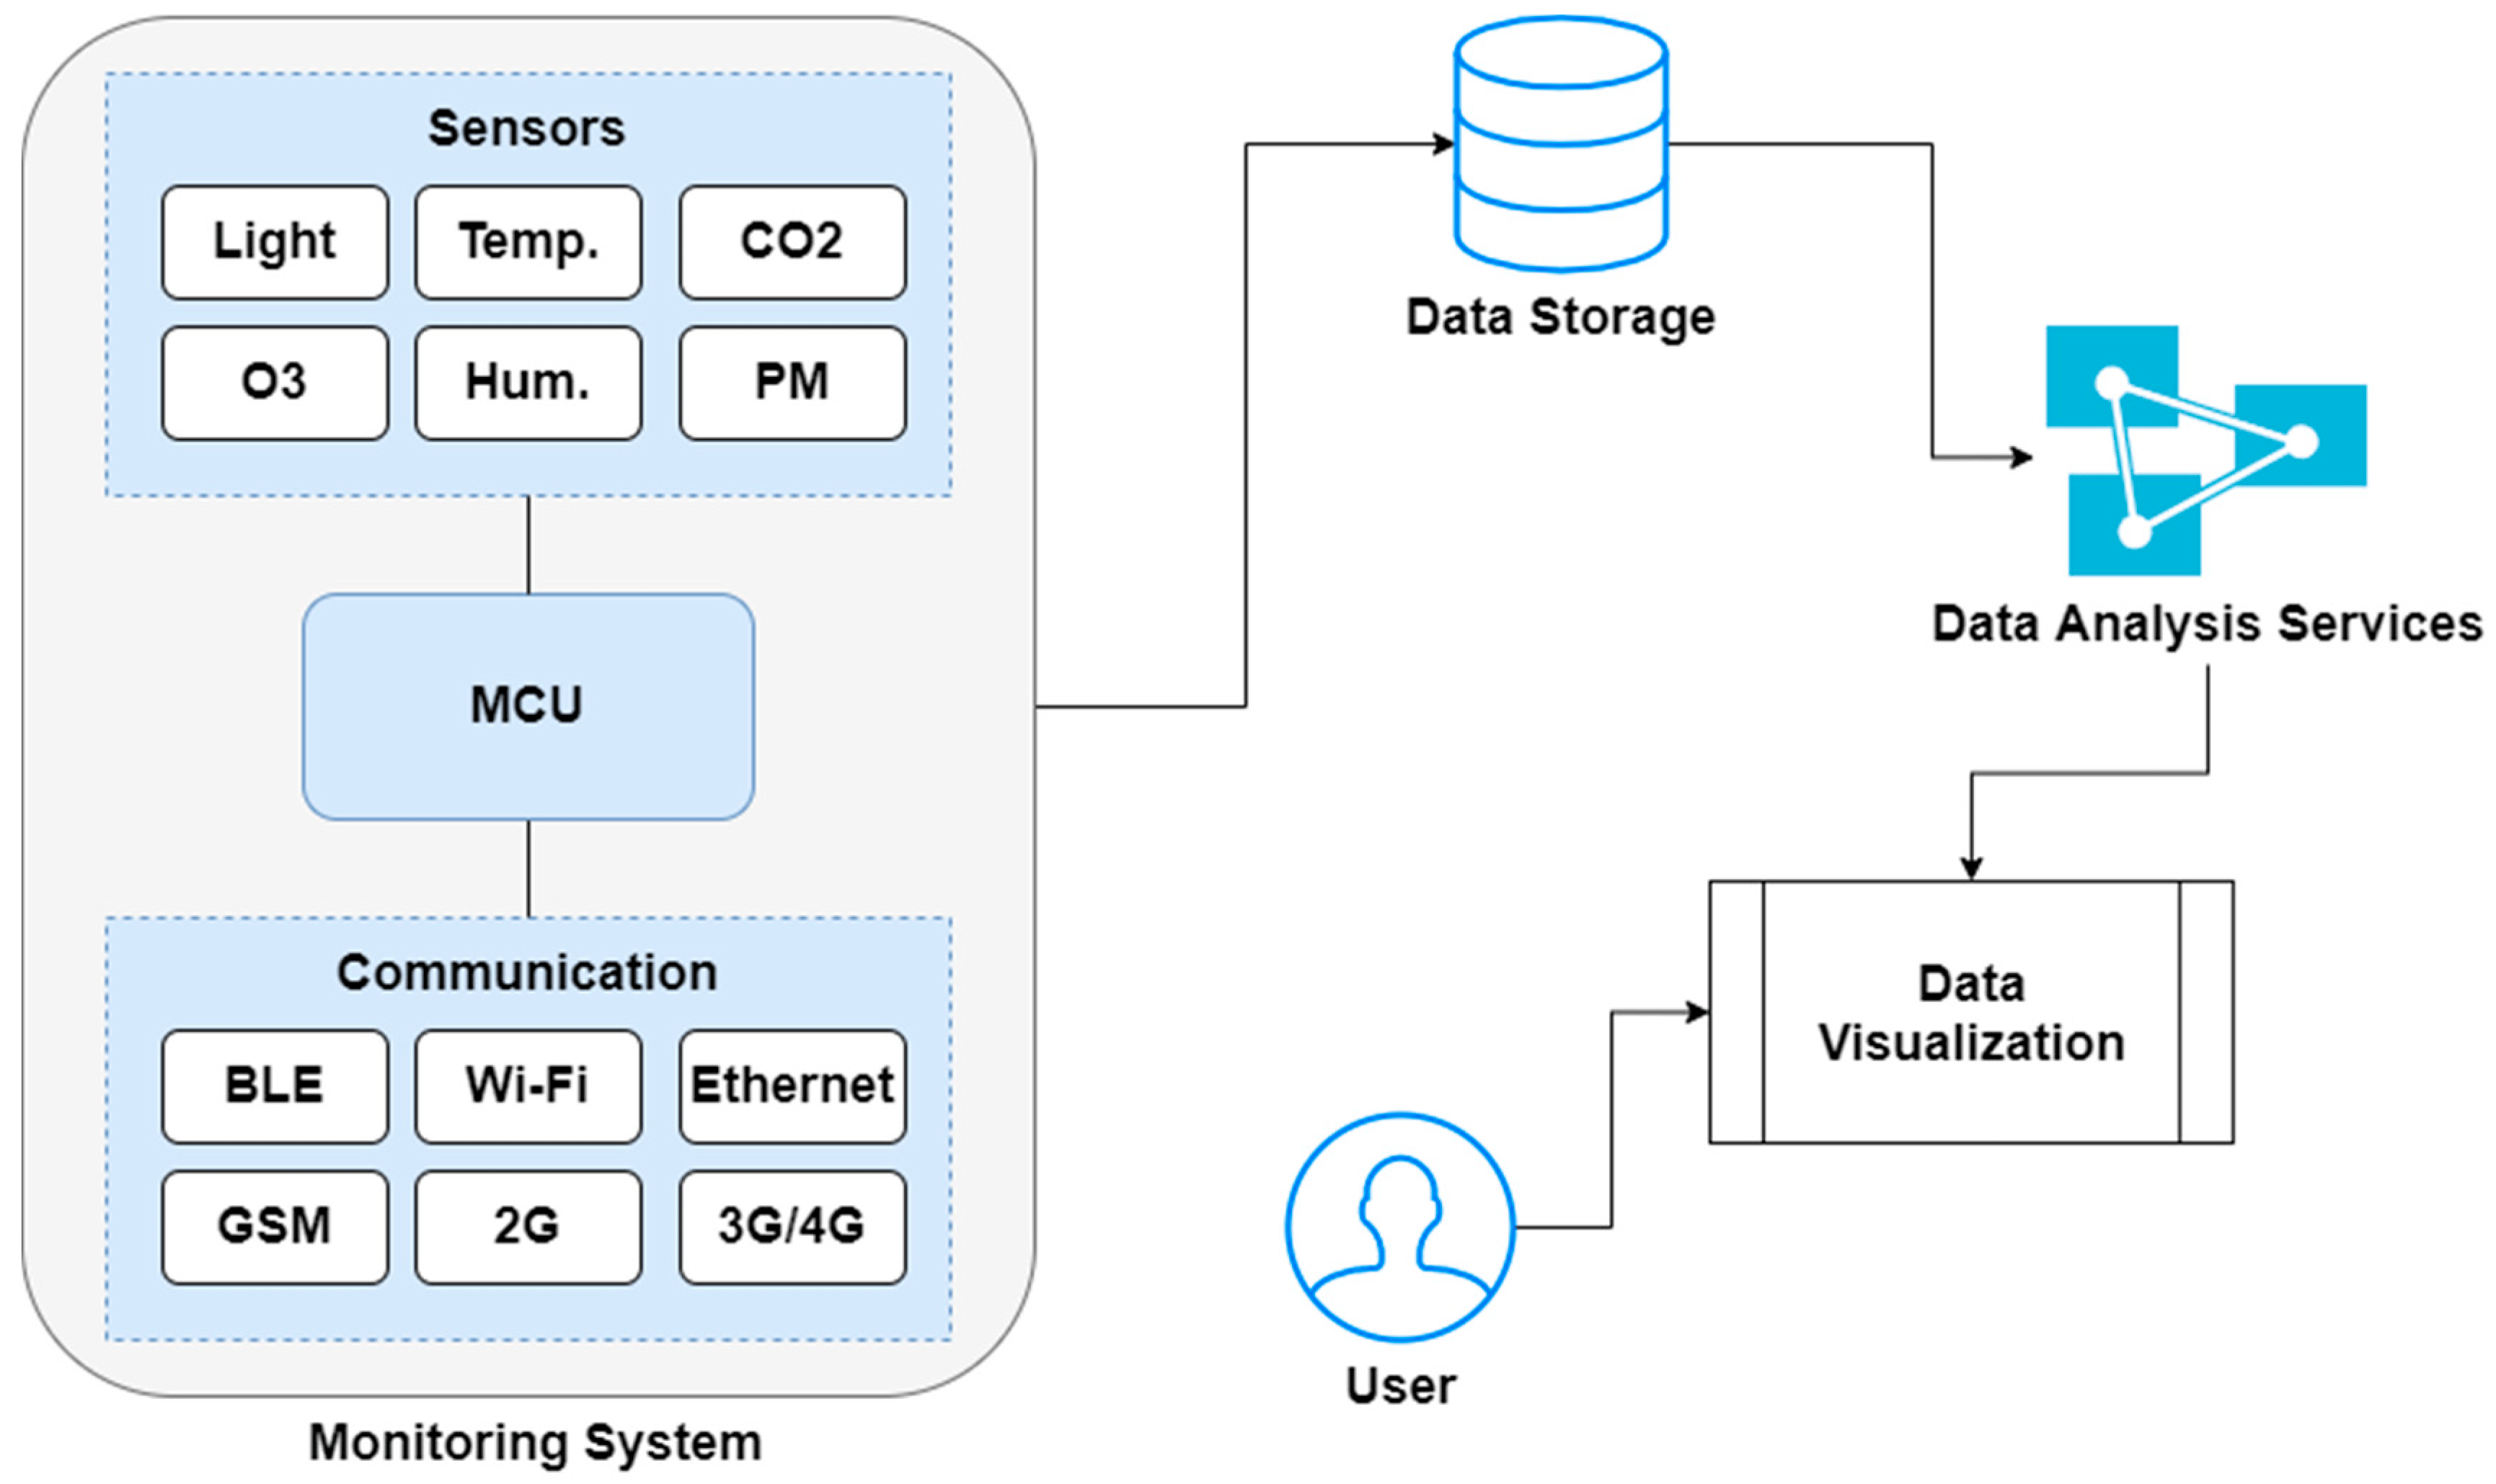
\includegraphics[width=0.7\linewidth]{images/Introduccion/general_architecture_of_internet_of_things_iot_based_iaq_monitoring_systems.png}
	\caption{\centering Arquitectura general para sistemas de monitoreo de IAQ basados en IoT. \cite{IAQ_monitoring_systems_based_on_internet_of_things_a_systematic_review}.}
	\label{fig: estructura_general_IoT}
\end{figure}


%1. Contexto general
    %1.1. Se presenta el tema general y se delimita el area de investigación
    %1.2. Teorias relevantes
        %1.2.0. Importancia de la medicion de CO2
        %1.2.1. Regulaciones vigentes para Co2
            %1.2.1. OMS
            %1.2.2. Nacional         
        %1.2.2. Beneficiones de IOT
            %1.2.1. Beneficios generales
            %1.2.2. Beneficios smart campus
        %1.2.3. Utilización del gateway
%2. Importancia del tema
    %2.1. Impacto en la salud y en la productividad 
    %2.2. Marco de desarrollo de sistemas de monitoreo en un smart campus
%3. Estado del conocimiento
    %3.1. Estudios previos de monitoreo de CO2
        %3.1.1. Sensores de mano
        %3.1.2. Red IOT
    %3.2. Brechas en investigación

%En el año 2022, se registraron robos en 19.1\% de las viviendas en Perú y que una de las causas con mayor porcentaje por la que no se realizó la denuncia, con 20.3\%, fue desconocer al delincuente.  Además, en el año 2022 se registraron 1347 denuncias de abigeato en Perú, un delito que se estipula como diferente tanto al robo como al hurto y consiste en el hurto de ganado \cite{INEIAnuario2018-2022}. También se han registrado casos de robos en centros agrícolas, que ponen en riesgo la vida de trabajadores y personal de seguridad \cite{adriana2023sistema}. Así como se han registrado robos en el sector agrícola y ganadero, también se han producido robos en el sector minero por parte de bandas delictivas que se infiltran en minas para robar oro y plata. Como se puede ver en el comunicado de la compañía minera Poderosa, las acciones para garantizar la seguridad de los trabajadores es urgente, pues a la fecha del comunicado 7 colaboradores de la empresa ya han sido asesinados por estas bandas delictivas \cite{poderosa-comunicado}. Estos incidentes vinculados al sector productivo se concentran principalmente en zonas rurales y territorios extensos, donde la presencia de personal de seguridad resulta escasa y la vigilancia se torna desafiante. Ante esta situación, resulta necesario implementar medidas para salvaguardar tanto a los trabajadores como a los activos de las empresas.

\introsection{Descripción de la situación problemática}

En los últimos años, la medición, el monitoreo y el cuidado de la calidad del aire han cobrado una creciente importancia. Tradicionalmente, el control de la calidad del aire exterior ha sido prioritario en áreas cercanas a fuentes de emisiones de gases nocivos y otros contaminantes. Sin embargo, investigaciones recientes han evidenciado los riesgos que representan los espacios cerrados con altas concentraciones de CO2 para la salud humana.

Tras la pandemia de SARS-CoV-2, que reveló múltiples vulnerabilidades y la falta de controles adecuados en instituciones sanitarias, hogares, centros educativos y laborales, el monitoreo de los niveles de CO2 ha adquirido una relevancia aún mayor. No solo por los efectos adversos de concentraciones elevadas de este gas en el organismo, sino también porque el CO2 es considerado un indicador clave del riesgo de contagio y proliferación de microorganismos en ambientes cerrados.

La necesidad de monitorear y controlar los niveles de CO2 ha llevado a un incremento significativo en los esfuerzos tanto a nivel nacional como internacional. Las autoridades e instituciones sanitarias están implementando medidas más rigurosas para abordar esta problemática. Un registro adecuado de estas mediciones no solo actúa como una medida preventiva, sino también como una respuesta inmediata en la protección de la calidad de vida de las personas y en la gestión de eventos de salud pública, como la mencionada pandemia.

%Desde hace años se ha dado cada vez mayor importancia a la medición, monitoreo y cuidado de la calidad de aire. Si bien es cierto, en lugares cercanos a emisiones de gases nocivos para el ser humano y otros contaminantes las medidas de monitoreo de la calidad del aire exterior han estado presente desde hace varios años; más recientemente, estudios han demostrado lo perjudicial que puede ser mantener espacios cerrados con altas concentraciones de CO2. 

%A día de hoy, tras la pandemia del SARS-CoV-2 que ha probado múltiples vulnerabilidades y ausencia de controles de salud tanto en las instituciones sanitarias, como en los hogares, y centros de estudio y trabajo, no solo es importante el monitoreo de los niveles de CO2 por los efectos de las altas concentraciones únicamente del mismo en el organismo, sino porque su medida es considerado un indicador de riesgo de contagio y proliferación de microorganismos en el ambiente.

%El monitoreo y posterior control de los niveles de CO2 es una necesidad que se debe y está siendo atendida con mayores esfuerzos en los últimos años. Esto se ve reflejado mediante la intervención de las autoridades e instituciones sanitarias tanto a nivel nacional, como internacional. El mantener un registro adecuado de estas mediciones no solo es una medida preventiva, sino una respuesta inmediata ante la protección de la calidad de vida de las personas y eventos de salud pública como la mencionada pandemia.





1. Descripción del problema
    1.1. ¿Qué se ha identificado? (altos niveles de CO2 en espacios cerrados)
    1.2. Evidencia y datos
        1.2.1. Estadisticas sobre concentración de CO2 en espacios cerrados
        1.2.2. Ejemplos y estudios en el que se hagan comparaciones
    1.3 Consecuencias
        1.3.1. Transmisión de enfermedades (Impacto en la salud)
        1.3.2. Menor productividad (Impacto en la productividad)


\introsection{Formulación del problema}

%El presente proyecto se centra en el diseño e implementación de una alternativa de robot de vigilancia y patrullaje capaz de identificar intrusos mediante procesamiento de imágenes. Para ello se escogió un robot de dos ruedas de tipo péndulo invertido, pues permite operar con mayor facilidad en espacios estrechos, y hacerlo con mayor rapidez que un robot de cuatro ruedas, lo que le permite adaptarse mejor a la estructura de las instalaciones en las que será usado \cite{TWR_advantages}. Para controlar el robot, se seleccionó el controlador adaptativo por modelo de referencia directo (MRAC directo) debido a que es un algoritmo de control robusto que permite controlar el robot sobre distintas superficies. Con respecto a los algoritmos de procesamiento de imágenes para patrullaje y detección de intrusos se seleccionó el clasificador Haar Cascade para detección de personas y el algoritmo de localización y el algoritmo de localización y mapeo simultáneos (SLAM) para ubicar el lugar las detecciones en el mapa de las instalaciones. Para incrementar la tasa de cuadros por segundo procesados, se implementó parte de los algoritmos de procesamiento de imágenes en lógica programable, es decir, circuitos lógicos secuenciales reconfigurables, como los FPGA (Field-Programmable Gate Arrays).

Dado el impacto de los altos niveles de CO2 en la salud y el rendimiento académico, especialmente en entornos cerrados como aulas, surge la pregunta: ¿Cómo podemos diseñar e implementar un sistema de monitoreo basado en IoT que mida, registre y alerte sobre los niveles de CO2 en tiempo real, asegurando que los ambientes educativos se mantengan dentro de los límites saludables establecidos?


\introsection{Objetivos de investigación}
En esta sección se presentan los objetivos de este Trabajo Final de Ingeniería Mecatrónica. Sobre ellos se estructuró la investigación y los resultados presentados.

\subsubsection*{Objetivo general}
Diseñar e implementar un sistema de monitoreo y alerta en tiempo real de niveles de CO\textsubscript{2} en aulas empleando comunicación inalámbrica LoRa en una red IoT.

\subsubsection*{Objetivos específicos}
\begin{enumerate}

\item Diseñar la arquitectura de la red IoT y la arquitectura de software de la aplicación de monitoreo de niveles de CO\textsubscript{2}.
\item Implementar la red de nodos sensores medidores de CO\textsubscript{2} basados en comunicación LoRa
\item Desarrollar una plataforma de software para la recolección, almacenamiento y visualización de los datos de CO\textsubscript{2} en tiempo real, y un sistema de alertas y notificaciones para informar a los usuarios sobre niveles críticos de CO\textsubscript{2}.
\item Realizar pruebas individuales y de integración para la red IoT y la aplicación de monitoreo.

\end{enumerate}

\introsection{Justificación}

%Desarrollar este proyecto permite contar con una alternativa de robot de patrullaje y vigilancia capaz de ejecutar el algoritmo de detección de intrusos en el mismo robot a una mayor tasa de cuadros por segundo gracias a la aceleración por hardware. Esta alternativa resulta particularmente útil para casos en los que el territorio extenso, no se cuenta con una red WI-FI local a la cual conectarse para hacer el procesamiento de imágenes en una computadora física y no es viable instalar un router portátil en el robot debido a que no hay cobertura de servicios de internet, como en zonas rurales, o no se desea enviar los datos a la nube para su procesamiento.

La calidad del aire en espacios cerrados ha adquirido gran importancia en los últimos años debido a los riesgos que altos niveles de CO2 representan para la salud humana y la productividad. Estudios recientes han demostrado que concentraciones elevadas de CO2 en interiores no solo afectan el rendimiento cognitivo y físico, sino que también son un indicador clave del riesgo de contagio y proliferación de microorganismos, un aspecto que ha cobrado relevancia tras la pandemia de SARS-CoV-2.

En el ámbito educativo, donde estudiantes y docentes pasan la mayor parte del tiempo en salones de clase, es esencial garantizar una adecuada calidad del aire. Sin embargo, muchos centros educativos no cuentan con sistemas de monitoreo que permitan medir en tiempo real los niveles de CO2, lo que puede derivar en ambientes no saludables que impactan negativamente tanto en el bienestar como en el rendimiento académico.

A pesar de los avances en tecnología IoT, la implementación de redes de monitoreo eficientes sigue siendo un reto. Este proyecto se enfoca en diseñar e implementar una red IoT de nodos sensores para medir los niveles de CO2 en aulas, recopilando esta información en una base de datos en la nube. El objetivo es poder alertar de manera oportuna cuando se sobrepasen los límites de CO2 permitidos, asegurando que el ambiente sea siempre apto para las personas, y así contribuir a la creación de entornos educativos más seguros y saludables, en línea con las regulaciones nacionales e internacionales vigentes sobre calidad del aire en interiores.


\introsection{Alcance y limitaciones}
%Este trabajo se centra en el diseño e implementación del algoritmo de control y los algoritmos de procesamiento de imágenes, mas no en la construcción del prototipo de robot móvil de dos ruedas. El prototipo utilizado para este proyecto es un prototipo a escala del robot de vigilancia. Con respecto a los algoritmos de procesamiento de imágenes, debido a que este proyecto se centra en la aceleración de estos algoritmos, no se lleva a cabo el entrenamiento de los algoritmos de procesamiento de imágenes. En este proyecto no se desarrolla el método por el cual el robot envía alertas de detección de intrusos, el cual podría utilizar tecnologías inalámbricas de largo alcance.

Este trabajo se enfoca en el diseño e implementación del sistema de monitoreo, incluyendo la arquitectura de software utilizada y la infraestructura de red requerida. No obstante, se trata de un prototipo, por lo que se desarrollará a una escala menor, la cual consta de tres nodos medidores, los cuales se ubicarán en tres salones de clase distintos, en lugar de desplegarse por todos los salones del campus. Con respecto a la arquitectura de software, se emplea como servidor de base de datos el mismo equipo mediante el cual se monitorean las lecturas de los nodos sensores. Por otra parte, no se contempla el diseño y fabricación de una carcasa protectora para los equipos electrónicos, la cual es necesaria para su uso continuo a largo plazo para proteger los equipos del deterioro provocado por la humedad de la zona. Con respecto al consumo energético, el reporte no se enfoca en la evaluación y optimización de los nodos sensores. Por último, se apunta a mejorar los aspectos del proyecto trabajados e incluir los nuevos mencionados en la continuación de su desarrollo.

\introsection{Organización del trabajo de investigación}
El plan de trabajo de esta investigación se muestra en la tabla \ref{tab: gantt}.

\begin{table}[H]
\centering
    \caption{\centering Diagrama de Gantt del proyecto.}
    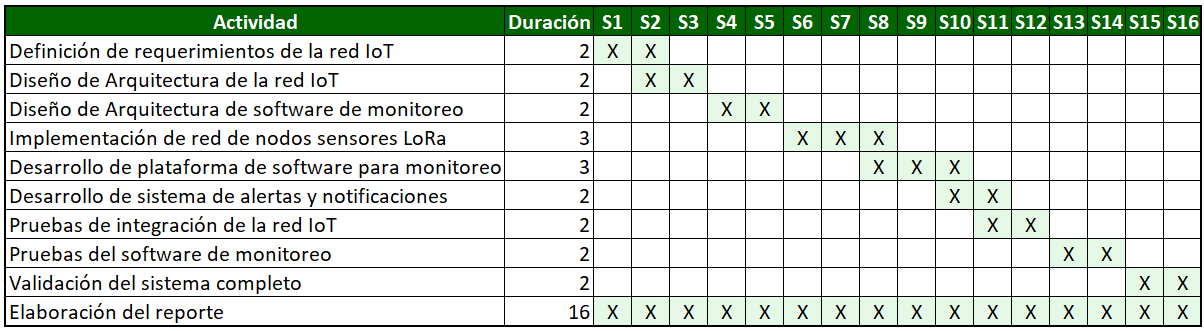
\includegraphics[width=1\linewidth]{images/Introduccion/Gantt.png}
\label{tab: gantt}
\end{table}

Este trabajo de investigación está organizado de la siguiente forma. El Capítulo I, la revisión de la literatura, presenta sistemas de medición y monitoreo de CO2 en espacios cerrados en proyectos de investigación como estado del arte e investigaciones relacionadas a herramientas de monitoreo manuales de CO2 u otros sistemas de medición de gases en espacios cerrados como trabajos previos. En el capítulo II, el marco teórico, se presenta tanto la arquitectura de la red IoT que contiene los nodos sensores, así como la arquitectura de software que se utilizará para el programa de monitoreo. En el Capítulo III, el marco metodológico, se presenta la implementación de red de nodos sensores LoRa, el desarrollo de la plataforma de software de monitoreo y el sistema de alertas y notificaciones. En el Capítulo IV, de resultados, se presentan las pruebas de integración de la red IoT, las pruebas del software de monitoreo y el sistema de alertas, y la validación del sistema completo. Por último, se abordan las conclusiones en relación con los objetivos planteados y se hacen recomendaciones para trabajos futuros.
